\documentclass[xcoler=dvipsnames, aspectratio=169]{beamer}

\usepackage{3191Style}
% Date gives the title of the lecture
\date{Systems of Linear Equations}

\begin{document}
\begin{frame}{Linear Equation Review}
    \begin{defn}
        Linear Equations:

        A linear equation of $n$ variables $x_1,\dots, x_n$ is an equation that can be written in the form
        \begin{equation*}
            a_1x_1 + a_2x_2 + \dots + a_nx_n = b
        \end{equation*}
        Where
        $b$ and $a_1,\dots,a_n$ are constants
    \end{defn}
    \pause
    \begin{practice}
        Determine which of the following equations are linear in $x_1,x_2,x_3$.

        \begin{columns}
            \column{.45\textwidth}
            \begin{enumerate}
                \item $x_1 + 4x_2 + x_1x_3 = 3$
                \item $\pi x_1 - \dfrac{x_2}{e^2} = 4$
            \end{enumerate}
            \column{.45\textwidth}
            \begin{enumerate}\addtocounter{enumi}{2}
                \item $\cos{(4)}x_1 + \sin{(2)}x_2 + x_3 = e\pi$
            \end{enumerate}
        \end{columns}
    \end{practice}
\end{frame}
\iftoggle{showSolutions}{
\begin{frame}{Linear Equation Review}
    \begin{defn}
        Linear Equations:

        A linear equation of $n$ variables $x_1,\dots, x_n$ is an equation that can be written in the form
        \begin{equation*}
            a_1x_1 + a_2x_2 + \dots + a_nx_n = b
        \end{equation*}
        Where
        $b$ and $a_1,\dots,a_n$ are constants
    \end{defn}
    \begin{practice}
        Determine which of the following equations are linear in $x_1,x_2,x_3$.

        \begin{columns}
            \column{.45\textwidth}
            \begin{enumerate}
                \item $x_1 + 4x_2 + x_1x_3 = 3$
                \item \alert{$\pi x_1 - \dfrac{x_2}{e^2} = 4$}
            \end{enumerate}
            \column{.45\textwidth}
            \begin{enumerate}\addtocounter{enumi}{2}
                \item \alert{$\cos{(4)}x_1 + \sin{(2)}x_2 + x_3 = e\pi$}
            \end{enumerate}
        \end{columns}
    \end{practice}
\end{frame}
}
{}
\begin{frame}{Systems of Linear Equations}
    \begin{defn}
        A \textit{system of linear equations} is a collection of many linear equations using the same variables
    \end{defn}
    \begin{ex}
        \begin{align*}
            2x_1 + 4x_2 &= 8 \\
            x_1 - 2x_2 &= 0
        \end{align*}
    \end{ex}
\end{frame}
\begin{frame}{A Linear System Solution Method}
    There are many ways that we learned to solve systems of linear equations in other math classes,
    the way we will discuss is called \textit{Elimination}. We will use this method to solve
        \begin{align*}
            2x_1 + 4x_2 &= 8 \\
            x_1 - 2x_2 &= 0
        \end{align*}
        \pause
    \[
        \begin{array}{c}
            2x_1 + 4x_2 = 8 \\
            1x_1 - 2x_2 = 0
        \end{array} 
        \rightarrow 
        \begin{array}{c}
            2x_1 + 4x_2 = 8 \\
            0x_1 - 4x_2 = -4
        \end{array}
        \pause
        \rightarrow
        \begin{array}{c}
            2x_1 + 0x_2 = 4\\
            0x_1 - 4x_2 = -4
        \end{array}
        \pause
        \rightarrow
        \begin{array}{c}
            1x_1 + 0x_2 = 2\\
            0x_1 + 1x_2 = 1
        \end{array}
    \]
    \pause
    So, our answer is \colorb{$(x_1,x_2) = (2,1)$}
    \pause
    \begin{rem}
        This method is called \textit{Elimination} because we are \textit{eliminating} variables until we
        only have one per equation!
    \end{rem}

\end{frame}
\begin{frame}{Looking At Our Solution Visually}
    % Image of desmos showing our lines intersecting at (2,1)
    \begin{center}
        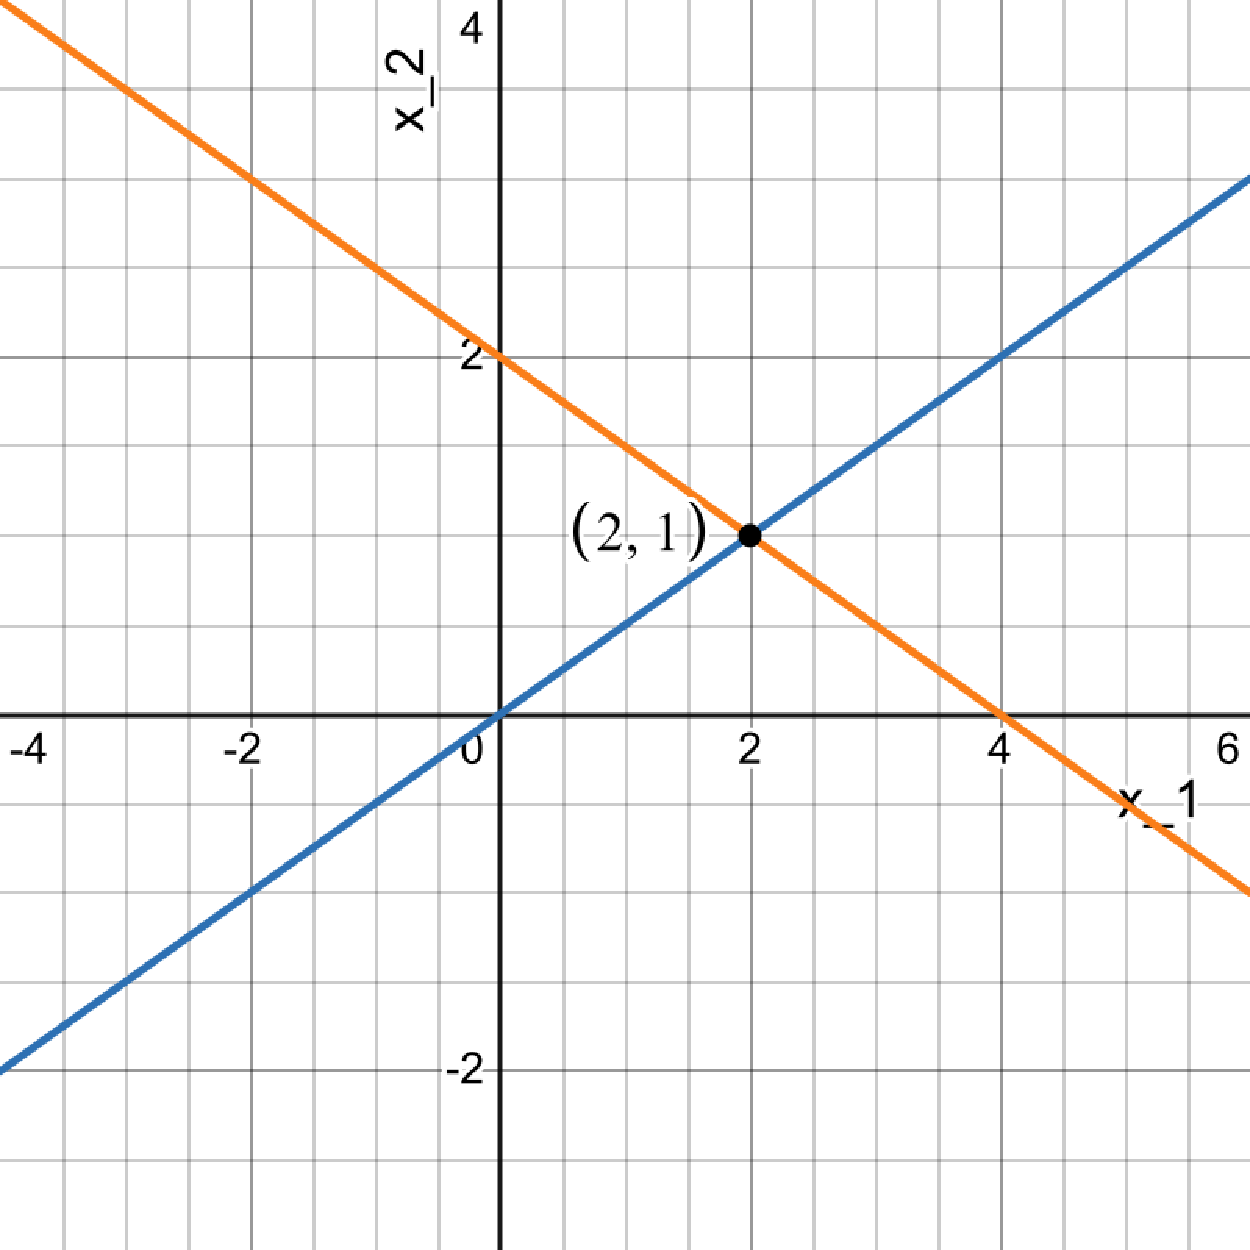
\includegraphics[height=.75\textheight]{images/oneSolution.pdf}
    \end{center}
\end{frame}
\begin{frame}{How Many Solutions Are There?}
    Let's consider two different linear systems
    \begin{columns}
        \column{.45\textwidth}
        \begin{align*}
            2x_1 + 4x_2 &= 4\\
            x_1 + 2x_2 &= 2
        \end{align*}
        \column{.45\textwidth}
        \begin{align*}
            2x_1 + 4x_2 &= 4\\
            x_1 + 2x_2 &= 4
        \end{align*}
    \end{columns}
    \pause
    % Images of these equations on desmos
    \begin{columns}
        \column{.45\textwidth}
            \begin{center}
                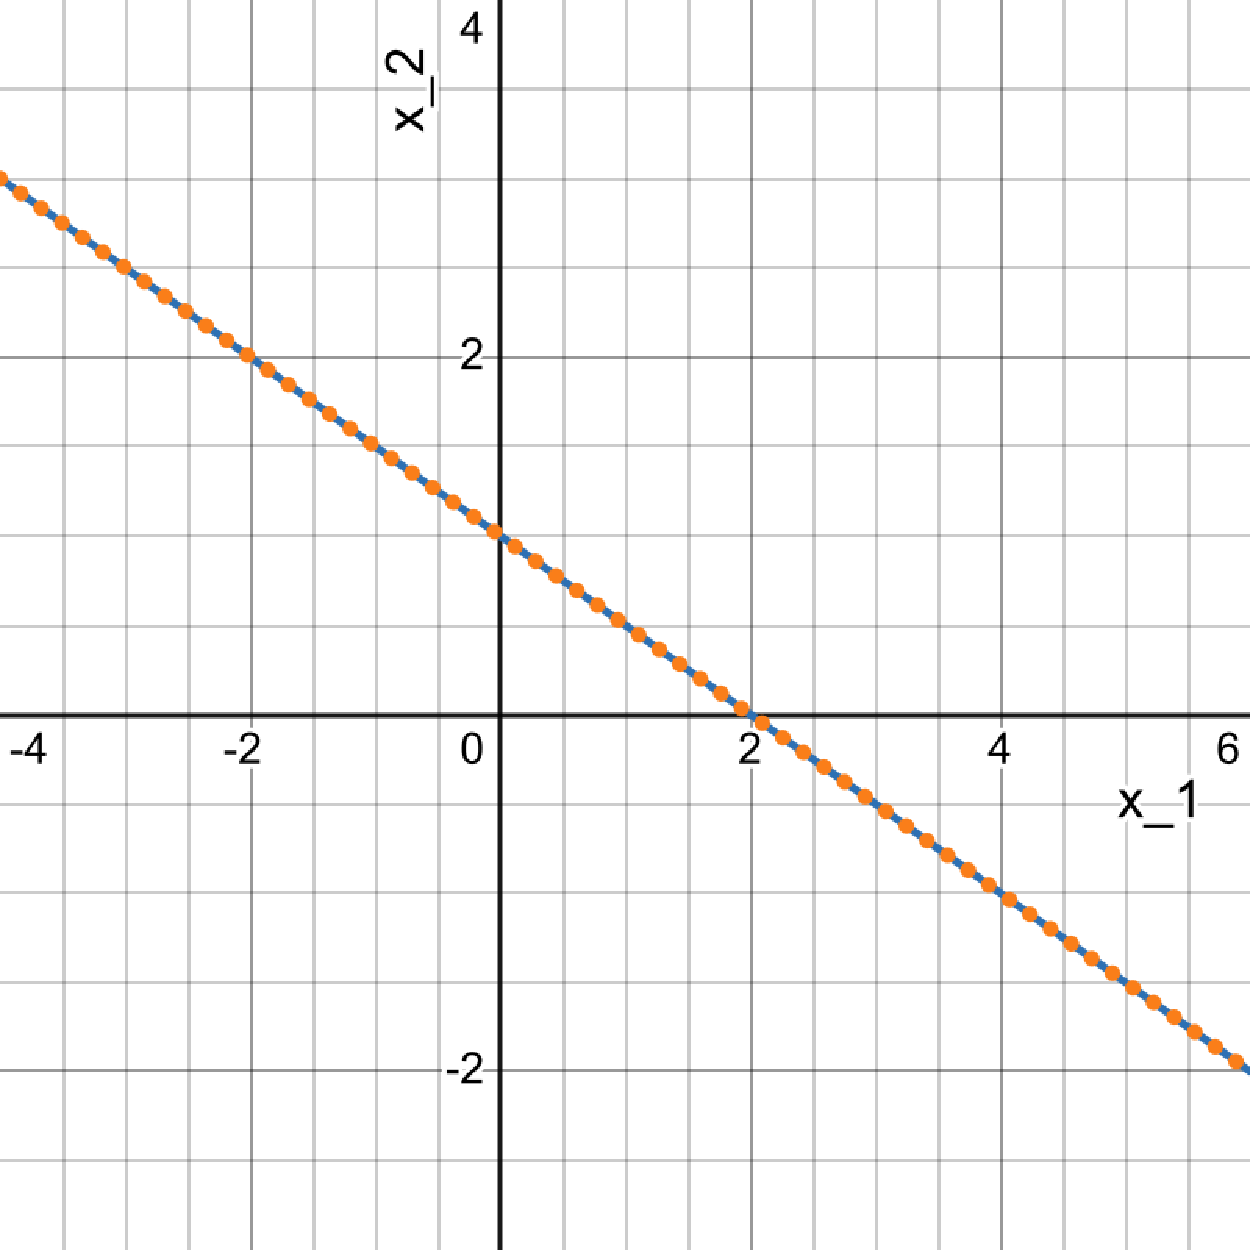
\includegraphics[height=.5\textheight]{images/infiniteSolutions.pdf}
            \end{center}
        \column{.45\textwidth}
            \begin{center}
                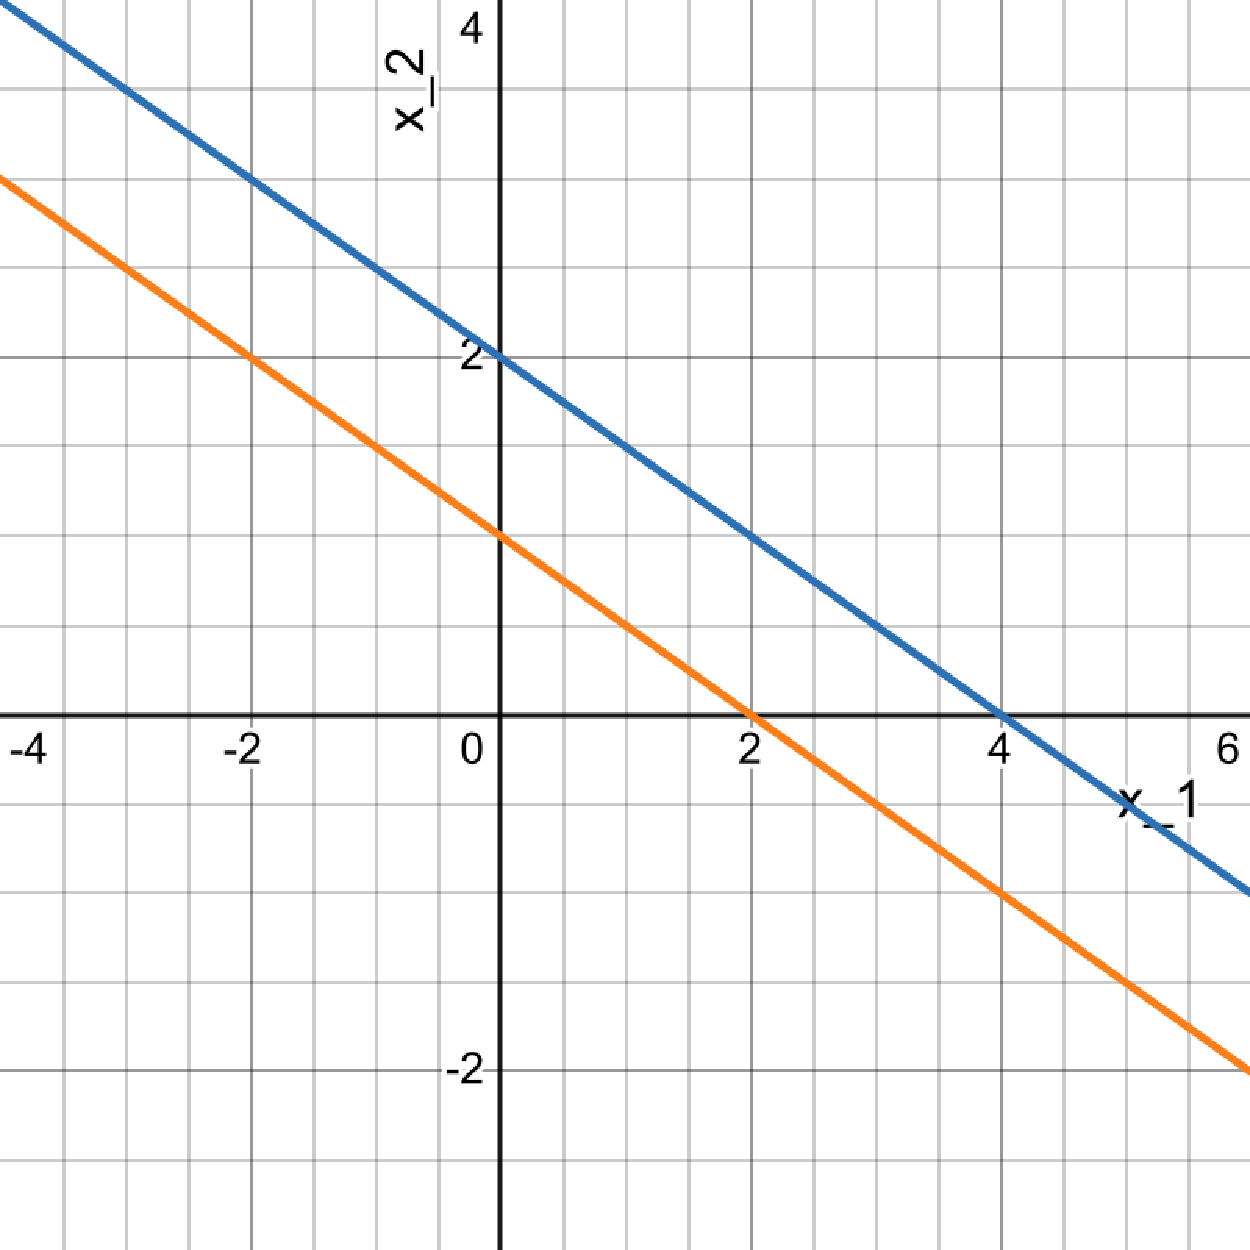
\includegraphics[height=.5\textheight]{images/noSolution.pdf}
            \end{center}
    \end{columns}
\end{frame}
\begin{frame}{Consistency}
    \begin{defn}
        A linear system of equations is called \textit{Consistent} if it has at least one solution, 
        and it is called \textit{Inconsistent} otherwise.
    \end{defn}
    \pause
    \begin{ex}
        From the previous slides, we would say that 
        \begin{columns}
            \column{.45\textwidth}
            \vspace{-.125in}
            \begin{align*}
                2x_1 + 4x_2 &= 4 \\
                x_1 + 2x_2 &=2
            \end{align*}
            \column{.45\textwidth}
            \vspace{-.125in}
            \begin{align*}
                2x_1 + 4x_2 &= 8 \\
                x_1 - 2x_2 &=0
            \end{align*}
        \end{columns}
        are consistent while
        \vspace{-.125in}
        \begin{align*}
            2x_1 + 4x_2 &= 4 \\
            x_1 + 2x_2 &=4
        \end{align*}
        is inconsistent.
    \end{ex}
\end{frame}
\begin{frame}{Consistency Practice}
    \begin{practice}
        Determine if the following systems are consistent or inconsistent
        \begin{columns}
            \column{.45\textwidth}
            \begin{enumerate}
                \item \begin{align*}
                        2x_1 + 4x_2 &= 1\\
                        4x_1 + 8x_2 &= 2
                \end{align*}
                \item \begin{align*}
                        6x_1 + 3x_2 &= 10\\
                        12x_1 + 6x_2 &= 10
                \end{align*}
            \end{enumerate}
            \column{.45\textwidth}
            \begin{enumerate}\addtocounter{enumi}{2}
                \item \begin{align*}
                        2x_1 + 3x_2 &=0 \\
                         x_1 + 5x_2 &= 0
                \end{align*}
                \item \begin{align*}
                        x_1 + x_2 &= 1\\
                        x_1 + x_2 &= 1
                \end{align*}
            \end{enumerate}
        \end{columns}
    \end{practice}
\end{frame}
\iftoggle{showSolutions}{
\begin{frame}{Consistency Practice Answers}
    \footnotesize
    \begin{practice}
        Determine if the following systems are consistent or inconsistent
        \begin{columns}
            \column{.45\textwidth}
            \begin{enumerate}
                \item \begin{align*}
                        2x_1 + 4x_2 &= 1\\
                        4x_1 + 8x_2 &= 2
                \end{align*}
                This system is consistent. It has an infinite number of solutions!
                \item \begin{align*}
                        6x_1 + 3x_2 &= 10\\
                        12x_1 + 6x_2 &= 10
                \end{align*}
                This system is inconsistent. There cannot be a solution
            \end{enumerate}
            \column{.45\textwidth}
            \begin{enumerate}\addtocounter{enumi}{2}
                \item \begin{align*}
                        2x_1 + 3x_2 &=0 \\
                         x_1 + 5x_2 &= 0
                \end{align*}
                This system is consistent. It has exactly 1 solution!
                \item \begin{align*}
                        x_1 + x_2 &= 1\\
                        x_1 + x_2 &= 1
                \end{align*}
                This system is consistent. It has an infinite number of solutions!
            \end{enumerate}
        \end{columns}
    \end{practice}
\end{frame}
}{}
\begin{frame}{Solution Set}
    \begin{defn}
        A \textit{solution set} is the set of all possible solutions to a system of 
        linear equations.
    \end{defn}
    \begin{ex}
        The solution set for the system \begin{align*}
                        x + y &= 1\\
                        x + y &= 1
                \end{align*}
                \pause
                would be
                $$\left.\left\{(x,y)\right|y = 1 - x\right\}$$
    \end{ex}
\end{frame}
\begin{frame}{Solution Set Practice}
    \begin{practice}
        Determine the solution set for each of the following systems
        \begin{columns}
            \column{.45\textwidth}
            \begin{enumerate}
                \item \begin{align*}
                        2x_1 + 4x_2 &= 1\\
                        4x_1 + 8x_2 &= 2
                \end{align*}
                \item \begin{align*}
                        6x_1 + 3x_2 &= 10\\
                        12x_1 + 6x_2 &= 10
                \end{align*}
            \end{enumerate}
            \column{.45\textwidth}
            \begin{enumerate}\addtocounter{enumi}{2}
                \item \begin{align*}
                        2x_1 + 3x_2 &=0 \\
                         x_1 + 5x_2 &= 0
                \end{align*}
            \end{enumerate}
        \end{columns}
    \end{practice}
\end{frame}
\iftoggle{showSolutions}{
\begin{frame}{Solution Set Practice Answers}
    \small
    \begin{practice}
        Determine the solution set for each of the following systems
        \begin{columns}
            \column{.45\textwidth}
            \begin{enumerate}
                \item \begin{align*}
                        2x_1 + 4x_2 &= 1\\
                        4x_1 + 8x_2 &= 2
                \end{align*}
                The solution set is
                    $\left.\left\{(x_1,x_2)\right|x_2 = \frac{1-2x_1}{4}\right\}$
                \item \begin{align*}
                        6x_1 + 3x_2 &= 10\\
                        12x_1 + 6x_2 &= 10
                \end{align*}
                The solution set is
                    $\emptyset$
            \end{enumerate}
            \column{.45\textwidth}
            \begin{enumerate}\addtocounter{enumi}{2}
                \item \begin{align*}
                        2x_1 + 3x_2 &=0 \\
                         x_1 + 5x_2 &= 0
                \end{align*}
                    The solution set is $\left\{(0,0)\right\}$.
            \end{enumerate}
        \end{columns}
    \end{practice}
\end{frame}
}{}
\begin{frame}{Matrix Notation}
    The way we've been writing our Elimination steps is pretty wasteful. Luckily for us, we
    have a way of doing this in a more space efficient method: a matrix!
    \vfill
    \pause
    \begin{columns}
        \column{.33\textwidth}
        System of linear equations:
        \begin{align*}
            \rTextWait{2}{3-}x_1 + \rTextWait{5}{3-}x_2 &= \bTextWait{1}{4-} \\
            \rTextWait{1}{3-}x_1 + \rTextWait{2}{3-}x_2 &= \bTextWait{7}{4-} 
        \end{align*}
        \pause
        \column{.33\textwidth}
        Coefficient Matrix:
        \[
            \begin{bmatrix}
                \rText{2} & \rText{5} \\
                \rText{1} & \rText{2}
            \end{bmatrix}
        \]
        \pause
        \column{.33\textwidth}
        Augmented Matrix:
        \[
            \aMat{cc|c}{
                \rText{2} & \rText{5} & \bText{1} \\
                \rText{1} & \rText{2} & \bText{7}
            }
        \]
        \pause
        or
        \[
            \begin{bmatrix}
                \rText{2} & \rText{5} & \bText{1}\\
                \rText{1} & \rText{2} & \bText{7}
            \end{bmatrix}
        \]
    \end{columns}
\end{frame}
\begin{frame}{Some Properties of Matrices}
    How many rows and columns does the following augmented matrix have?
    \[
        \onslide<2->\rText{3}\left\{\rule{0cm}{21pt}\right.\onslide<3-> \underbrace{ \onslide<1->\aMat{cccc|c}{
            2 & 9 & 13 & 3 & 0 \\
            1 & 0 & 2  & 1 & 1 \\
            4 & 1 & 0  & 2 & 12
        }\onslide<3-> }_{\bText{5}}
    \]
    \pause
    \begin{itemize}
        \item This matrix has \rText{3} rows. This means there were $3$ equations in the original system
            \pause
        \item This matrix has \bText{5} columns. This means there were $4$ variables in the original system
            \pause
        \item We would say this is a $\rText{3}\times \bText{5}$ augmented matrix.
    \end{itemize}
            \pause
    Note: The order is very important when we use the shorthand, \rText{rows} always comes first and 
    \bText{columns} always go second.
\end{frame}
\begin{frame}{Solving a Linear System With Matrices}
    \only<1>{
    Let's look at how we can use this augmented matrix by solving a system our old way and the 
    new way simultaneously}
    \footnotesize
    \begin{columns}
        \column{.5\textwidth}
        \only<2->{
        \begin{align*}
            2x_1 + 4x_2 &= 8 \\
            1x_1 - 2x_2 &= 0
        \end{align*}
        }
        \only<4->{
        \vspace{-15pt}
        \begin{align*}
            2x_1 + 4x_2 &= 8 \\
            0x_1 - 4x_2 &= -4
        \end{align*}
        }
        \only<6->{
        \vspace{-15pt}
        \begin{align*}
            2x_1 + 0x_2 &= 4 \\
            0x_1 - 4x_2 &= -4
        \end{align*}
        }
        \only<8->{
        \vspace{-15pt}
        \begin{align*}
            1x_1 + 0x_2 &= 2 \\
            0x_1 + 1x_2 &= 1
        \end{align*}
        }
        \column{.5\textwidth}
        \only<3->{
            \[
                \aMat{cc|c}{
                    2 & 4 & 8 \\
                    1 &-2 & 0
                }
            \]
        }
        \only<5->{
            \vspace{-15pt}
            \begin{center}
                $R_2=R_2 - \frac{1}{2}R_1$
            \end{center}
            \vspace{-5pt}
            \[
                \aMat{cc|c}{
                    2 & 4 & 8 \\
                    0 &-4 & -4
                }
            \]
        }
        \only<7->{
            \vspace{-15pt}
            \begin{center}
                $R_1=R_1 + R_2$
            \end{center}
            \vspace{-5pt}
            \[
                \aMat{cc|c}{
                    2 & 0 & 4 \\
                    0 &-4 & -4
                }
            \]
        }
        \only<9->{
        \vspace{9pt}
            \vspace{-20pt}
            \begin{center}
                $R_1=\frac{1}{2}R_1$, $R_2 = -\frac{1}{4}R_2$
            \end{center}
            \vspace{-5pt}
            \[
                \aMat{cc|c}{
                    1 & 0 & 2 \\
                    0 & 1 & 1
                }
            \]
        }
    \end{columns}
\end{frame}
\begin{frame}{A Larger System!}
    \begin{practice}
        Solve the following system of equations for $x_1,x_2,x_3$ 
        \begin{align*}
            x_1 + x_2 + x_3 &= 7\\
            x_1 - x_2 + 2x_3 &= 7\\
            5x_1 + x_2 + x_3 &= 11
        \end{align*}
    \end{practice}
\end{frame}
\iftoggle{showSolutions}{
\begin{frame}{A Larger System Solution}
    \[
        \aMat{ccc|c}{
            1 & 1 & 1 & 7 \\
            1 &-1 & 2 & 7 \\
            5 & 1 & 1 &11
        }\rightarrow\aMat{ccc|c}{
            1 & 1 & 1 & 7 \\
            0 &-2 & 1 & 0 \\
            5 & 1 & 1 &11
        }\rightarrow\aMat{ccc|c}{
            1 & 1 & 1 & 7 \\
            0 &-2 & 1 & 0 \\
            0 &-4 &-4 &-24
        }\rightarrow
    \]
    \pause
    \[
        \aMat{ccc|c}{
            1 & 1 & 1 & 7 \\
            0 &-2 & 1 & 0 \\
            0 & 0 &-6 &-24
        }\rightarrow\aMat{ccc|c}{
            1 & 1 & 1 & 7 \\
            0 &-2 & 1 & 0 \\
            0 & 0 & 1 & 4
        }\rightarrow\aMat{ccc|c}{
            1 & 1 & 1 & 7 \\
            0 &-2 & 0 &-4 \\
            0 & 0 & 1 & 4
        }\rightarrow\aMat{ccc|c}{
            1 & 1 & 1 & 7 \\
            0 & 1 & 0 & 2 \\
            0 & 0 & 1 & 4
        }\rightarrow
    \]
    \pause
    \[
        \aMat{ccc|c}{
            1 & 0 & 1 & 5 \\
            0 & 1 & 0 & 2 \\
            0 & 0 & 1 & 4
        }\rightarrow\aMat{ccc|c}{
            1 & 0 & 0 & 1 \\
            0 & 1 & 0 & 2 \\
            0 & 0 & 1 & 4
        }
    \]
    \pause
    So, our solution is $\bText{(x_1,x_2,x_3)} = \bText{(1,2,4)}$
\end{frame}
}{}
\begin{frame}{Elementary Row Operations}
    \small
    We have a name for the kinds of changes we are making to these matrices, we call them
    ``Elementary Row Operations''
    \pause
    \begin{defn}
        An operation on a row of a matrix called is an Elementary Row Operation if it is one of
        \begin{enumerate}
            \item \rTextWait{Replacement}{2,6}: Replace one row by itself plus a multiple of another row
                \pause
            \item \bTextWait{Interchange}{3,7}: Swap two rows
                \pause
            \item \rTextWait{Scaling}{4,8}: Multiply an entire row by the same constant
        \end{enumerate}
    \end{defn}
    \pause
    \begin{example}
        \[
            \aMat{ccc|c}{
                1 & -8 & 0 & 6\\
                0 &  0 & 2 & 8\\
                0 &  1 & 0 &-3
            }\pause\rightarrow\aMat{ccc|c}{
                \rTextWait{1}{6} & \rTextWait{0}{6} & \rTextWait{0}{6} &\rTextWait{-18}{6}\\
                0 &  0 & 2 & 8\\
                0 &  1 & 0 &-3
            }\pause\rightarrow\aMat{ccc|c}{
                1 &  0 & 0 &-18\\
                \bTextWait{0}{7} & \bTextWait{1}{7} & \bTextWait{0}{7} & \bTextWait{-3}{7}\\
                \bTextWait{0}{7} & \bTextWait{0}{7} & \bTextWait{2}{7} & \bTextWait{8}{7}
            }\pause\rightarrow\aMat{ccc|c}{
                1 &  0 & 0 &-18\\
                0 &  1 & 0 &-3\\
                \rTextWait{0}{8} & \rTextWait{0}{8} & \rTextWait{1}{8} & \rTextWait{4}{8}
            }
        \]
    \end{example}
\end{frame}
\begin{frame}{Equivalent Systems}
    \begin{defn}
        Two matrices (augmented or not augmented) are Row Equivalent if we can transform them into
        each other using only Elementary Row Operations
    \end{defn}
    \pause
    \begin{example}
        \[
            \aMat{ccc|c}{
                1 & -8 & 0 & 6\\
                0 &  0 & 2 & 8\\
                0 &  1 & 0 &-3
            }\text{ and }\aMat{ccc|c}{
                1 &  0 & 0 &-18\\
                0 &  1 & 0 &-3\\
                0 &  0 & 1 & 4
            }
        \]
        are Row Equivalent augmented matrices.
    \end{example}
    \pause
    \begin{rem}
        If two augmented matrices are row equivalent, then the solutions to their respective 
        systems are the same!
    \end{rem}
\end{frame}
\begin{frame}{Equivalent Systems}
    \begin{defn}
        Two linear systems are called Equivalent if they have the same solution.
    \end{defn}
    \pause
    \begin{example}
        \begin{columns}
            \column{.5\textwidth}
            \begin{align*}
                2x_1 + 4x_2 &= 2\\
                1x_1 + 3x_2 &= 5
            \end{align*}
            \column{.5\textwidth}
            \begin{align*}
                4x_1 + 8x_2 &= 4\\
                2x_1 + 6x_2 &= 10
            \end{align*}
        \end{columns}
        Are equivalent systems because the right one is just the left with both rows multiplied by $2$.
    \end{example}
\end{frame}
\end{document}
